\apendice{Plan de Proyecto Software}

\section{Introducción}

En el siguiente apéndice se realizará una estimación de tiempo, trabajo y dinero que será necesario invertir para al realización de este proyecto.

En una primer apartado se tratará sobre la evolución temporal que ha tenido el proyecto, indicando los principales cambios y objetivos de cada \emph{Sprint}, así como una estimación del tiempo que se estimaba, seria necesario invertir antes de la realización del mismo.

En la segunda parte se centra en la viabilidad del proyecto tanto en el ámbito económico (estimación de costes y beneficios) como en el legal (licencias software, etc.). 

%En el siguiente apéndice se incluye la evolución temporal que ha tenido del proyecto durante la realización del mismo, además de aspectos relevantes de diseño y económicos que afectarán a su viabilidad.	

\section{Planificación temporal}

En este apartado se procederá a explicar con detalle cuál ha sido el resultado de la planificación del proyecto. Esta planificación se ha realizado utilizando una metodología ágil basada en \emph{sprints} de una duración de una o dos semanas en función de las necesidades y el tiempo disponible debido a otras cargas de trabajo diferentes a este proyecto.

En estos \emph{sprints} se van marcando ciertos objetivos que serán revisados junto a los tutores en las reuniones al final de los mismos. Los objetivos del siguiente \emph{sprint} serán marcados durante dichas reuniones.

Para el control de tiempos se ha utilizado la herramienta ZenHub siendo la valoración de los \emph{Story Points} la siguiente:

\tablaSmall{Equivalencias \emph{Story Points} y tiempo estimado}{c c }{StoryPoints/tiempo}
{ \multicolumn{1}{l}{Story Points} & Estimación temporal \\}{ 
	1            & 1 hora              \\ 
	2            & 1,5 horas           \\ 
	3            & 2 horas             \\ 
	4            & 2,5 horas           \\ 
	5            & 3 horas             \\ 
	6            & 3,5 horas           \\ 
	7            & 4 horas             \\ 
	8            & 6 horas             \\ 
	9            & 9 horas             \\ 
}

%Aclarar que los gráficos \emph{Burn Down} de los primeros \emph{sprints} no están todo lo bien que deberían por la poca experiencia con la herramienta.

\subsection{Sprint 1 (29/01/2020 - 05/02/2020)}\label{Sprint-1}
En esta primera reunión se marcó el comienzo del proyecto. Ya se había hablado anteriormente con uno de los tutores (José Francisco) del interés sobre el proyecto propuesto del que también formaba parte de los tutores Álvar Arnaiz.

Al ser la primera reunión se habló de las herramientas que se iban a utilizar así como acordar los primeros objetivos de este \emph{sprint}:

\begin{itemize}
\item Crear el repositorio.
\item Añadir la plantilla de \LaTeX{} a la documentación.
\item Crear cuenta en la plataforma \emph{Copernicus}.
\item Investigar el funcionamiento básico de las librerías a utilizar.
\item Leer una serie de papers que me proporcionaron sobre las medusas.
\end{itemize}

Las \emph{issues} para este \emph{Sprint} se pueden ver \href{https://github.com/psnti/TFG-Pablo-Santidrian-Tudanca/milestone/1}{aquí}.

Se estimó unas 10 horas de trabajo de las que finalmente se invirtieron 8 horas quedando sin terminar una \emph{issue}.

\imagen{Sprint1_BurnDown.png}{\textit{Burndown chart} del Sprint 1}

\subsection{Sprint 2 (13/02/2020 - 28/02/2020)}\label{Sprint-2}

En la segunda reunión se comentó la existencia de una API para la descarga de los datos meteorológicos como alternativa a la descarga de una gran cantidad de datos a través del FTP.

Por otro lado, se me proporcionaron apuntes de la asignatura de minería de datos para su lectura y aprendizaje.

Por último, los tutores me recomendaron iniciar la documentación del plan de proyecto de los \emph{Sprints} que se fuesen sucediendo para no acumular trabajo y se pudiera olvidar detalles del mismos.

Los objetivos fueron los siguientes:

\begin{itemize}
\item Realizar script para la descarga de los datos.
\item Comenzar a documentar el plan del proyecto.
\item Lectura de apuntes y papers.
\end{itemize}

Las \emph{issues} para este \emph{Sprint} se pueden ver \href{https://github.com/psnti/TFG-Pablo-Santidrian-Tudanca/milestone/2}{aquí}.

Se estimaron unas 8 horas de trabajo de las que finalmente se invirtieron 9 horas.

\imagen{Sprint2_BurnDown.png}{\textit{Burndown chart} del Sprint 2}

\subsection{Sprint 3 (28/02/2020 - 17/03/2020)}\label{Sprint-3}

En esta tercera reunión hablamos sobre la descarga de los datos, de las dos opciones posibles nos quedamos con la descarga por FTP por ser más fiable. Además este \emph{Sprint} se centrará en su mayor parte en documentación como las herramientas a utilizar o cuestiones teóricas sobre las medusas aparte de comenzar a desarrollar la base de la aplicación web.

Se marcaron los siguientes objetivos:
\begin{itemize}
\item Comienzo desarrollo web.
\item Elaboración de parte de la documentación teórica.
\item Descarga de los datos en un equipo de cómputo habilitado en la Universidad.
\end{itemize}

Las \emph{issues} para este \emph{Sprint} se pueden ver \href{https://github.com/psnti/TFG-Pablo-Santidrian-Tudanca/milestone/3}{aquí}.

Se estimó unas 19 horas y finalmente se realizaron 24. La causa del desvió de horas principalmente fueron: el comienzo del desarrollo web por el desconocimiento previo y el comentar el código creado para la descarga de los datos necesarios pues se corrigieron errores y se mejoró la salida por pantalla con una barra de descarga más visual.


\imagen{Sprint3_BurnDown.png}{\textit{Burndown chart} del Sprint 3}

\subsection{Sprint 4 (17/03/2020 - 30/03/2020)}\label{Sprint-4}

La cuarta reunión se hizo mediante \emph{Skype} con José Francisco debido a la cuarentena por el coronavirus. Se habló sobre la necesidad de utilizar la VPN de la universidad por este mismo motivo para poder tener acceso a la maquina remota. 

Por otra parte, se mostró el avance de la web acordando que el siguiente paso debería ser la introducción de los mapas para lo que se comentaron varias bibliotecas de las que se podía hacer uso.

Los objetivos que se marcaron fueron:
\begin{itemize}
	\item Continuación desarrollo web.
	\item Introducción de mapas en la aplicación web.
	\item Conexión a la VPN de la universidad para conseguir dejar los datos descargándose aunque la sesión esté cerrada.
	\item Continuación de la documentación.
\end{itemize}

Las \emph{issues} para este \emph{Sprint} se pueden ver \href{https://github.com/psnti/TFG-Pablo-Santidrian-Tudanca/milestone/4}{aquí}.

\imagen{Sprint4_BurnDown.png}{\textit{Burndown chart} del Sprint 4}

Se estimaron 15 hora y media y finalmente se realizaron 16.

\subsection{Sprint 5 (30/03/2020 - 14/4/2020)}\label{Sprint-5}

Esta reunión se realizó también de manera remota por \emph{Skype} con ambos tutores. Se mostró la implementación de los mapas en la aplicación web así como varias mejoras en la interfaz de la misma. También avances realizados en la memoria y ciertas mejoras propuestas por los tutores.

Sobre la web, a pesar de haber empezado su desarrollo, se recomendó el realizar unos bocetos de la misma para definir la estructura a seguir.

Por otro lado, una vez descargados los datos oceánicos, el siguiente paso será generar una estructura de datos para poder entrenar al modelo.

Por último, se acordó que el siguiente paso en la realización de la memoria debía ser la finalización de los objetivos del proyecto y definir los requisitos.

Los objetivos que se marcaron fueron los siguientes:
\begin{itemize}
	\item Generar estructura de datos.
	\item Definir objetivos del proyecto.
	\item Definir requisitos.
	\item Definir aspectos relevantes.
	\item Realizar bocetos aplicación web.
\end{itemize}

Las \emph{issues} para este \emph{Sprint} se pueden ver \href{https://github.com/psnti/TFG-Pablo-Santidrian-Tudanca/milestone/5}{aquí}.

\imagen{Sprint5_BurnDown.png}{\textit{Burndown chart} del Sprint 5}

Se estimaron 12,5 horas y finalmente se realizaron 18,5.

\subsection{Sprint 6 (15/4/2020 - 24/4/2020)}\label{Sprint-6}

%Comentarios reunión.
En esta reunión se mostraron los avances realizados en la generación de la estructura de datos que posteriormente se utilizará en la creación del modelo de predicción. Se comentaron diferentes problemas encontrados como la existencia de valores nulos es los datos de origen así como la mejor forma de localizar los cuadrantes contiguos a las playas.\\
También se realizaron cambios en la memoria y anexos.

Para este sprint se marcaron como objetivo:
\begin{itemize}
	\item Añadir más cuadrantes a la estructura de datos mencionada así como asegurar la selección de los cuadrantes contiguos a las playa.
	\item Redacción de casos de uso.
	\item Investigar el despliegue de la página web.
	\item Añadir diferentes partes  documentación.
\end{itemize} 

Las \emph{issues} para este \emph{Sprint} se pueden ver \href{https://github.com/psnti/TFG-Pablo-Santidrian-Tudanca/milestone/6}{aquí}.

%Gráfico
\imagen{Sprint6_BurnDown.png}{\textit{Burndown chart} del Sprint 6}

%Estimación horas
En un principio se estimaron 16 horas y media y finalmente se realizaron 21 horas.

\subsection{Sprint 7 (25/4/2020 - 8/5/2020)}\label{Sprint-7}

%Comentarios reunión.
La temática de la reunión de este sprint fue similar a la anterior. Se habían solucionado los problemas con los valores nulos y añadido más cuadrantes a la estructura de datos, esto dio lugar a algunos problemas por la orientación de las playas. Por este motivo se revisarán las playas para ver si es posible reducir el numero de las mismas y así hacer un predicción más precisa.\\
En relación a esto, se empezará con la realización del modelo predictivo aprendiendo la utilización de la biblioteca \emph{Scikit-Learn}.
Por último, se mostró el auto despliegue de la aplicación web con \emph{heroku} desde un repositorio a parte del original.

Para este sprint se marcaron como principales objetivos:
\begin{itemize}
	\item Mejoras en la interfaz de la aplicación web.
	\item Revisar los datos obtenidos de las playas para reducir el dataset inicial si fuese necesario.
	\item Aprender la utilización de \emph{Scikit-learn}.
	\item Corrección y ampliación de anexos y memoria.
\end{itemize} 

Las \emph{issues} para este \emph{Sprint} se pueden ver \href{https://github.com/psnti/TFG-Pablo-Santidrian-Tudanca/milestone/7}{aquí}.

%Gráfico
\imagen{Sprint7_BurnDown.png}{\textit{Burndown chart} del Sprint 7}

%Estimación horas
En un principio se estimaron 20 horas y finalmente se realizaron 27.

\subsection{Sprint 8 (12/5/2020 - 2/6/2020)}\label{Sprint-8}

Esta reunión se basó principalmente en la realización del modelo. Se comentaron algunas correcciones en la estructura de los datos (valores nulos, desfase temporal en la organización de los avistamientos).

Por otra parte, hablamos de diferentes algoritmos de minería de datos que se podría utilizar para realizar pruebas y con los que se obtienen mejores resultados así como otras transformaciones que realizar a la estructura de datos para lograr mejores resultado como la normalización de los datos o dar más importancia a unas clases que a otras.

Para este sprint se marcaron como principales objetivos:
\begin{itemize}
	\item Arreglos en la estructura de datos.
	\item Investigar los diferentes algoritmos.
	\item Probar algoritmos de minería de datos.
	\item Documentar las pruebas y teoría de minería de datos.
\end{itemize} 

Las \emph{issues} para este \emph{Sprint} se pueden ver \href{https://github.com/psnti/TFG-Pablo-Santidrian-Tudanca/milestone/8}{aquí}.

%Gráfico
\imagen{Sprint8_BurnDown.png}{\textit{Burndown chart} del Sprint 8}

%Estimación horas
En un principio se estimaron 12 horas y finalmente se realizaron 20.

\subsection{Sprint 9 (3/6/2020 - 10/6/2020)}\label{Sprint-9}
La reunión estuvo basada en los algoritmos de predicción a utilizar. Se mostraron los diferentes algoritmos probados con algunos resultados y se propuso por parte de los tutores la prueba de alguno más.

Aparte de esto, hablamos sobre la posibilidad de utilizar series temporales debido a la naturaleza de los datos. También se obtuvo un nuevo conjunto de datos con un mayor número de lecturas de las que se tenía hasta el momento.


Para este sprint se marcaron como principales objetivos:
\begin{itemize}
	\item Seguir realizando pruebas con diferentes algoritmos de minería.
	\item Investigar sobre las series temporales.
	\item Tratar nuevo Excel.
\end{itemize} 

Las \emph{issues} para este \emph{Sprint} se pueden ver \href{https://github.com/psnti/TFG-Pablo-Santidrian-Tudanca/milestone/9}{aquí}.

%Gráfico
\imagen{Sprint9_BurnDown.png}{\textit{Burndown chart} del Sprint 9}

%Estimación horas
En un principio se estimaron 14 horas y finalmente se realizaron 22 hora y media.

\subsection{Sprint 10 (10/6/2020 - 17/6/2020)}\label{Sprint-10}

La temática de la reunión fue la misma que las anteriores. Las pruebas realizadas aplicando las series temporales a los modelos no aportaron buenos resultados por lo que se decidió realizar estas con validación cruzada y ver que algoritmo arroja mejores resultados.

En cuanto a la página web, se mostró la introducción de algunas funcionalidades viendo que existían bugs que subsanar.

Para este sprint se marcaron como principales objetivo:
\begin{itemize}
	\item Pruebas de algoritmos con validación cruzada.
	\item Arreglar fallos e introducir gráfico en la página web.
\end{itemize} 

Las \emph{issues} para este \emph{Sprint} se pueden ver \href{https://github.com/psnti/TFG-Pablo-Santidrian-Tudanca/milestone/10}{aquí}.

%Gráfico
\imagen{Sprint10_BurnDown.png}{\textit{Burndown chart} del Sprint 10}

%Estimación horas
En un principio se estimaron 18 horas y finalmente se realizaron 41.

\subsection{Sprint 11 (17/6/2020 - 24/6/2020)}\label{Sprint-11}

En primer lugar, se trató la realización de las ultimas pruebas realizadas con los modelos. Se obtuvo un resultado aceptable por lo que será el modelo a introducir finalmente en la pagina web. 

Por otra parte, se mostraron los avances en la aplicación web que estaba casi terminada por completo. Se propuso por parte de los tutores la introducción de un nuevo gráfico mostrando un historial de los avistamientos en la playa seleccionada. En cuanto a la forma de introducir el modelo, se barajaron varias formas. Finalmente se subirán una serie de los datos de origen con los que pueda trabajar el modelo.

Para este sprint se marcaron como principales objetivos:
\begin{itemize}
	\item Finalizar la aplicación web.
	\item Dejar finalizada la documentación a falta de la revisión final por parte de los tutores.
\end{itemize} 

Las \emph{issues} para este \emph{Sprint} se pueden ver \href{https://github.com/psnti/TFG-Pablo-Santidrian-Tudanca/milestone/11}{aquí}.

%Gráfico
\imagen{Sprint11_BurnDown.png}{\textit{Burndown chart} del Sprint 11}

%Estimación horas
En un principio se estimaron 34 horas y finalmente se realizaron 43.

\subsection{Sprint 12 (17/6/2020 - 24/6/2020)}\label{Sprint-11}

Este \emph{Sprint} se centró principalmente en la realización de la documentación. Se finalizó casi por completo y fue revisada por los tutores. A parte se realizaron unas ultimas mejoras en la pagina web a falta de introducir el modelo final.

Para este sprint se marcaron como principales objetivo:
\begin{itemize}
	\item Finalizar las correcciones de la documentación.
	\item Introducir el modelo final en la aplicación web.
	\item Realizar los vídeos de las entregas.
	\item Mejorar lo \emph{Readme} de ambos repositorios.
	\item Generar \emph{release}.
\end{itemize} 

Las \emph{issues} para este \emph{Sprint} se pueden ver \href{https://github.com/psnti/TFG-Pablo-Santidrian-Tudanca/milestone/12}{aquí}.

%Gráfico
\begin{figure}[!h]
	\centering
	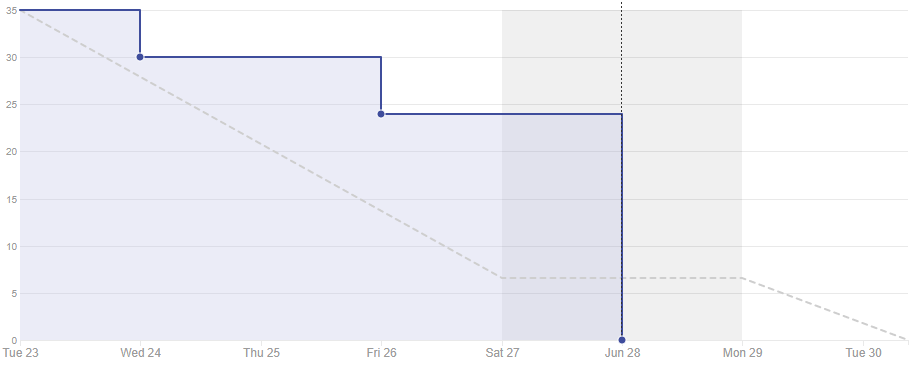
\includegraphics[width=0.8\textwidth]{Sprint12_BurnDown.png}
	\caption{\textit{Burndown chart} del Sprint 11}\label{}
\end{figure}


%Estimación horas
En un principio se estimaron 20,5 horas y finalmente se realizaron 24,5.

\subsection{Resumen}

\section{Estudio de viabilidad}

\subsection{Viabilidad económica}

\subsection{Costes}
\subsubsection{Coste software}
Todas las herramientas software utilizadas son de uso gratuito por lo que el coste de este apartado es cero.
\subsubsection{Coste hardware}
El coste de dispositivos es bajo. Se ha utilizado un ordenador personal valorado en 800 euros. Suponiendo una amortización de 5 años, el coste amortizado seria:

\begin{equation}
\frac{800}{12 * 5} * 5 = 66,67  \text{\euro}
\end{equation}

También se utilizó la máquina de cómputo de la Universidad que tuvo un coste inicial de 4350 euros con una amortización de 6 años.

\begin{equation}
\frac{4350}{12 * 6} * 5 = 322,91  \text{\euro}
\end{equation}

El coste total del hardware será de 389,58 euros.

\subsubsection{Coste de personal}

Se considera que el proyecto se ha realizado por un desarrollador trabajando 6 horas diarias durante 5 meses:


\begin{table}[H]
	\begin{center}
		\begin{tabular}{ll}
			\hline
			Concepto                        & Coste (€) \\ \hline
			Salario bruto del trabajador    & 1200      \\
			Contingencias comunes (23,6 \%) & 283,2     \\
			Desempleo (5,5 \%)              & 66        \\
			Fogasa (0,2 \%)                 & 2,4       \\
			Formación profesional (0,6 \%)  & 7,2       \\ \hline
			Coste total mensual             & 1558,80  
		\end{tabular}
	\end{center}
\end{table}


El coste del empleado seria de 1558,80 euros mensuales. Si aplicamos esto por los 5 meses de trabajo el coste total del personal ascendería a 7794€.

\subsection{Beneficios}
El proyecto esta realizado para ser disfrutado de manera gratuita y sin publicidad, por lo que a corto plazo no se obtendrían beneficios. Se podría plantear la posibilidad de agregar algunas funcionalidades extras a futuro, siendo estas de pago a través de algún tipo de suscripción mensual.

\subsection{Viabilidad legal}

Para la realización del proyecto se han utilizado multitud de biblioteca de Python de dominio público. A continuación, en la tabla \ref{tabla:Licencias}, se expondrán las principales herramientas utilizadas.


\begin{table}%[H]
	\centering
	\caption{Licencias de bibliotecas y herramientas utilizadas}
	\label{tabla:Licencias}
	\rowcolors {2}{gray!35}{}
	\begin{tabular}{l l l l}
		\toprule
		Librería     & Versión & Descripción                                                     & Licencia                \\ 	\midrule	
		VsCode        & 1.46.1  & \begin{tabular}[c]{@{}l@{}}Editor de código.\\  \end{tabular} & MIT\\ 
		Jupyter Notebook & 	6.0.3 & \begin{tabular}[c]{@{}l@{}}Aplicación para el desarrollo de \\código en múltiples lenguajes.\\  \end{tabular} & BSD\\
		Scikit-Learn & 0.22.1  & \begin{tabular}[c]{@{}l@{}}Biblioteca para aprendizaje\\ automático en Python.\end{tabular}	               & BSD                     \\
		Flask       & 1.1.1     &  \begin{tabular}[c]{@{}l@{}}Biblioteca para crear\\ aplicaciones web en Python. \end{tabular}               & BSD    \\
		Jinja2       & 2.11.1     &  \begin{tabular}[c]{@{}l@{}} Motor para integrar Python \\ con documentos HTML. \end{tabular}               & BSD                     \\
		Folium       & 0.11.0     &  \begin{tabular}[c]{@{}l@{}}Biblioteca para generar mapas \\en Python \end{tabular}               & MIT                     \\
		tmux       & 3.1b     &  \begin{tabular}[c]{@{}l@{}}Multiplexador de terminales. \end{tabular}               & ISC                     \\
		Bootstrap    & 3.3.7.1    & \begin{tabular}[c]{@{}l@{}}Biblioteca para desarrollar\\ aplicaciones web responsive.\end{tabular}                      & MIT  	\\
		JQuery    & 3.2.1    & \begin{tabular}[c]{@{}l@{}}Biblioteca para optimizar\\ JavaScript.\end{tabular}
		& MIT                 \\
		Morris.js    & 0.5.1    & \begin{tabular}[c]{@{}l@{}}Biblioteca para crear\\ gráficos en Javascript y HTML.\end{tabular}                     
		& MIT \\ \bottomrule
	\end{tabular}
\end{table}

Teniendo en cuenta todas estas, la licencia final del proyecto es MIT (Massachusetts Institute Technology) siendo una licencia de uso libre y permitiendo su uso comercial y modificación.

